\documentclass[12pt]{article}
\usepackage[margin=0.75in]{geometry}
\geometry{letterpaper}
\usepackage[T1]{fontenc} % Support Icelandic Characters
\usepackage[utf8]{inputenc} % Support Icelandic Characters
\usepackage{graphicx} % Support for including images
\usepackage{hyperref} % Support for hyperlinks

%Color
\usepackage{color}
\definecolor{nred}{RGB}{19,40,81}
\definecolor{nblue}{RGB}{86,99,146}
\definecolor{nalgo}{RGB}{188,139,76}
\usepackage{sectsty}
\sectionfont{\color{nred}}
\subsectionfont{\color{nblue}}
\subsubsectionfont{\color{nalgo}}

%Cabeceras
\usepackage{fancyhdr}
\pagestyle{fancy}
\fancyhead[L]{Runge-Kutta}
\fancyhead[C]{Facultad de Ingeniería y Arquitectura}
\fancyhead[R]{Universidad de Oriente}
%------------------------------------------------------------------
% TITLE
%------------------------------------------------------------------
\title{
\centerline{
\includegraphics[width=90mm]{images/UNIVO.png}}
\vspace{0.5 cm}
Método Runge-Kutta
\large  \\
\vspace{1.0 cm}
Análisis Numérico\\ 
\small Universidad De Oriente - Facultad de Ingeniería y Arquitectura, Ciudad Universitaria, San Miguel 
  }

\author{
    Jorge Sánchez\\
    \texttt{sanchez503jorge@gmail.com}\\\\
    Hugo Bénitez\\
    \texttt{correo@gmail.com}
}

\date{\today}


%------------------------------------------------------------------
% DOCUMENT START HERE
%------------------------------------------------------------------
\begin{document}
\maketitle
\begin{titlepage}
	\tableofcontents{}
\end{titlepage}

\section*{Introducción}
\newpage


\section{EL PROBLEMA}

\subsection{Titulo descriptivo del proyecto}

\subsection{Planteamiento del problema}

\subsection{Enunciado del problema}

\subsection{Justificación}
En el campo de la Ingeniería, y en particular de la Ingeniería en Sistemas, se presentan muchos fenomenos 
físicos que necesitan representarse mediante modelos matemáticos, algunos de los cuales 
no son faciles de resolver a partir de métodos análiticos y en algunos casos es imposible 
obtener una solucion y en otros, ésta implica procesos complejos que para fines prácticos resultan incovenientes.

\subsection{Delimitaciones}

\subsubsection{Teorías}
Método de Runge-Kutta

El método de Runge-Kutta es un método genérico de resolución numérica de Ecuaciones Diferenciales.\\

El método de Runge-Kutta no es soló un único método, sino una importante familia de métodos iterativos, tanto implícitos como explícitos, 
para aproximar las soluciones de Ecuaciones Diferenciales ordinarias (E.D.Ós); estas 
tecnicas fueron desarrolladas alrededor de 1900 por los matemáticos alemanes Carl David Tolmé Runge y Martin Wilhelm Kutta.
El más popular de los métodos RK es el de cuarto orden. Como en el caso de los proce-
dimientos de segundo orden, hay un número infinito de versiones. La siguiente, es la
forma comúnmente usada y, por lo tanto, le llamamos método clásico RK de cuarto
orden:\\
\\
$y_{i+1}=y_i+\frac{1}{6}(k_1+2k_2+2k_3+k_4)h $\\
\\
\textbf{Donde:}\\
\\
$k_1=f({x_i,y_i})$\\
\\
$k_2=f(x_i+\frac{1}{2}h,y_i+\frac{1}{2}k_1h)$\\
\\
$k_3=f(x_i+\frac{1}{2}h,y_i+\frac{1}{2}k_2h)$\\
\\
$k_4=f(x_1+h,y_i+k_3h)$
\begin{center}
  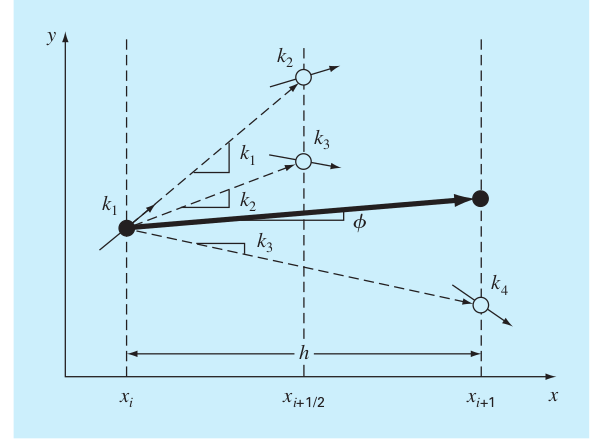
\includegraphics[width=100mm]{images/Figura1.png}\\
  \textbf{Representación gráfica de las pendientes estimadas empleadas en el método RK de cuarto
  orden.}
\end{center}
Observe que con las EDO que están en función sólo de x, el método RK clásico de
cuarto orden es similar a la regla de Simpson 1/3. Además, el método RK de cuarto
orden tiene similitud con el procedimiento de Heun en cuanto a que se usan múltiples
estimaciones de la pendiente para obtener una mejor pendiente promedio en el interva-
lo. Como se muestra en la figura 1, cada una de las k representa una pendiente. La
ecuación 2, entonces representa un promedio ponderado de éstas para establecer
la mejor pendiente.
\subsection{Objetivos}

\subsubsection{General}
Aprender a resolver Ecuaciones Diferenciales lineales de cuarto orden a través del método de Runge-Kutta.
\subsubsection{Especificos}
\begin{enumerate}
	\item Conocer ventajas y desventajas del método.
	\item Comparar el método de Runge-Kutta con la solución de la Ecuación resuelta por métodos de integración.
	\item Identificar la exactitud del método.
\end{enumerate}

\section{FUNDAMENTACION TEÓRICA}

\section{METODOLOGÍA}
\end{document}
